\subsection*{Item 1}

O diagrama da constelação apresenta no eixo complexo os símbolos de um sinal modulado, com as componentes em fase no eixo das abscissas e as componentes em quadratura no eixo das ordenadas. O sinal NRZ bipolar apresentado no problema possui dois símbolos distintos, sendo eles $\{-1, 1\}$ no eixo real.

O sinal transmitido e que não possui influência do AWGN apresenta um diagrama de constelação perfeito, ou seja, para uma quantidade n de bits transmitidos, os possíveis símbolos só ocuparão a posição -1 e 1 do eixo em fase do diagrama de constelação. A figura \ref{fig:clean} considera

\begin{figure}[H] 
\centering
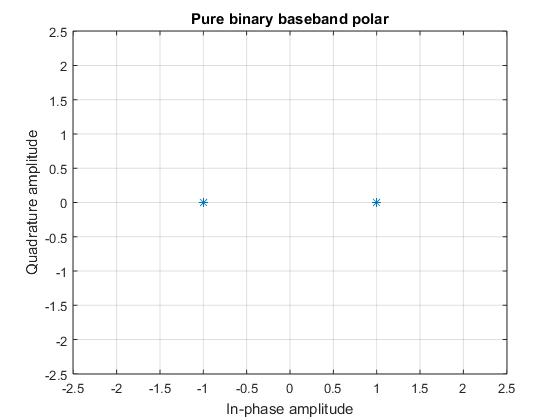
\includegraphics[width=8cm]{images/item1_clean.jpg}
\caption{Constelação do sinal banda base polar livre de ruído.}
\label{fig:clean} 
\end{figure}

Porém ao considerar o canal AWGN com característica probabilística e complexa, haverá uma significativa mudança na constelação do sinal recebido. Essa mudança fará com que os símbolos que antes estavam centrados em -1 e 1 no eixo em fase, agora flutuem em torno desses valores possuindo componentes em fase e em quadratura, assim gerando uma nuvem em torno dos símbolos pretendidos.

Uma figura de mérito deve ser levada em conta para destacar quantitativamente quanto a potência do sinal se destaca da potência do AWGN, pois se a potência do ruído for muito relevante em relação à potência do sinal, a nuvem em torno dos símbolos do diagrama de constelação pode aumentar e confundir a detecção a respeito de qual a posição original dos símbolos.

Um parâmetro conhecido em comunicações digitais e que funciona como uma boa figura de mérito para o sinal é a relação entre energia do bit pela densidade espectral de potência do ruído, o $E_bN_0$ $\left(\frac{E_b}{N_0}\right)$. Sua influência na constelação diz respeito diretamente ao quão dispersa será a nuvem de símbolos em torno dos símbolos originalmente transmitidos. Um alto $E_bN_0$ significa que a potência do sinal se destaca da potência do ruído e gera uma nuvem mais contido em torno dos símbolos originais, enquanto que o contrário gera uma nuvem dispersa que pode causar erro na detecção dos símbolos.

Um exemplo da influência do $E_bN_0$ na constelação pode ser observado graficamente na figura \ref{fig:noisy}, que apresenta uma mesma quantidade de bits sendo transmitida em duas condições de $E_bN_0$.

\begin{figure}[H]
\begin{center}
    \subfigure[$E_bN_0 = 5dB$]{             
        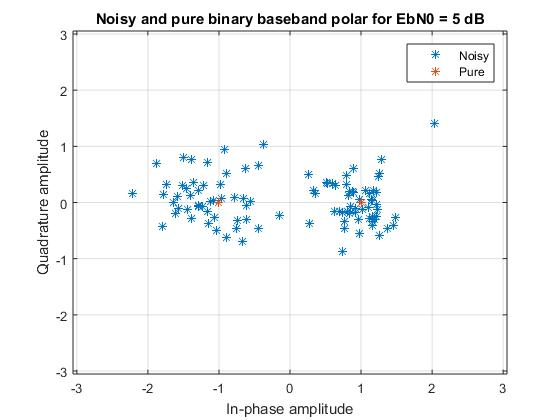
\includegraphics[width=7.5cm]{images/item1_a.jpg}  
        \label{fig:noisy1a}
    }
    \subfigure[$E_bN_0 = 10dB$]{                                              
        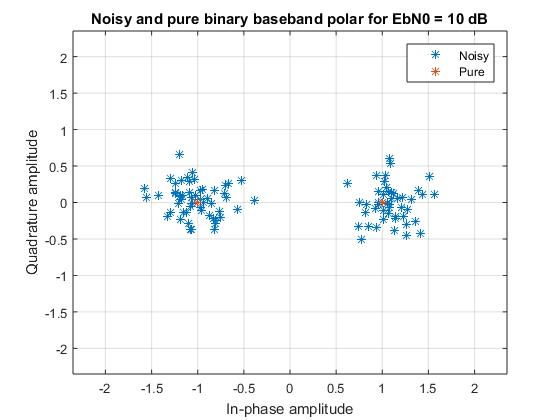
\includegraphics[width=7.5cm]{images/item1_b.jpg}
        \label{fig:noisyb}
    }                
\end{center}
\caption{Comparação entre sinal transmitido e recebido na na entrada de um receptor sujeito AWGN em diferentes condições de $E_bN_0$.}
\label{fig:noisy} 
\end{figure}

Assim permite-se traçar graficamente comparações com a constelação do sinal transmitido (não influenciado pelo ruído), uma vez que esta está sobreposta à constelação do sinal recebido.

\subsection*{Item 2}

Agora considerando a transmissão para vários valores de $E_bN_0$ diferentes, pode-se observar a progressão do diagrama de constelação. Sua tendência é tornar a nuvem mais concentrada em torno dos símbolos -1 e 1, de acordo com que $E_bN_0$ aumenta e elimina ambiguidades na detecção (diminuir o erro de detecção).

Com a transmissão e detecção para diferentes valores de $E_bN_0$ permite-se traçar um gráfico da taxa de erro de bits (BER) em função do $E_bN_0$. Esse gráfico da $E_bN_0$ $\times$ BER é uma versão quantizada do gráfico da probabilidade de erro teórica ($P_e$) em função de $E_bN_0$. A $P_e$ é encontrada a partir da função Q ou da função complementar do erro (erfc).

Um gargalo para encontrar uma BER que corresponda ao valor da $P_e$ é a quantidade de bits transmitida. Como a $P_e$ depende unicamente da $E_bN_0$, seu valor será preciso para cada valor de $E_bN_0$ fornecido. Porém a BER depende do número de bits transmitido e ela será precisa para valores menores de probabilidade de erro apenas para um alto número de bits transmitidos.

Por exemplo, considerando o caso da transmissão de 1000 bits, a quantidade máxima de bits detectados incorretamente serão 500 bits. Isso, pois um valor maior que 50\% para a taxa de erros significaria que uma inversão no dispositivo de decisão seria o bastante para manter a taxa novamente abaixo do limite 50\%. Como a quantidade de bits é um valor inteiro, a resolução da BER para esse caso será valores de 1/1000 (0.1\%) de espaçamento. Se for considerar a curva da BER para valores baixos como $10^{-6}$ ou $10^{-7}$, para o caso de 1000 bits não haverá precisão o suficiente para diferenciar entre esses dois valores. Assim, a solução possível para esse problema é aumentar a quantidade de bits transmitidos.

\begin{figure}[H]
\begin{center}
    \subfigure[$10^3 bits$]{             
        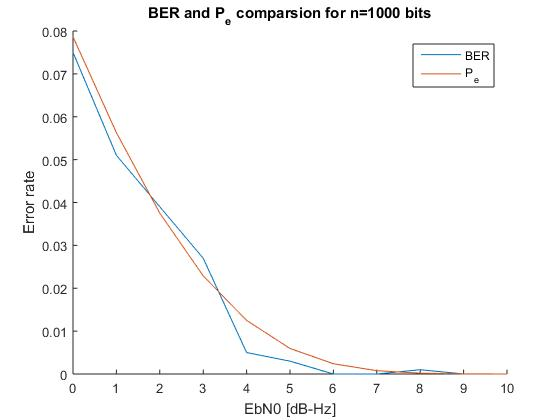
\includegraphics[width=7.5cm]{images/item2a.jpg}  
        \label{fig:item2a}
    }
    \subfigure[$10^4 bits$]{             
        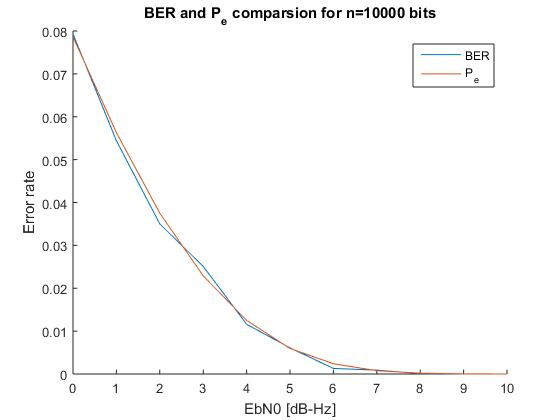
\includegraphics[width=7.5cm]{images/item2b.jpg}  
        \label{fig:item2a}
    }
    \subfigure[$10^5 bits$]{             
        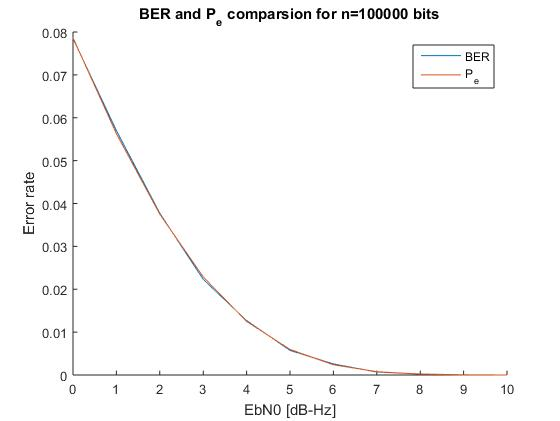
\includegraphics[width=7.5cm]{images/item2c.jpg}  
        \label{fig:item2a}
    }
         
\end{center}
\caption{Curva de probabilidade de erro teórica em comparação com a taxa de erro de bits estimada pela transmissão de \{$10^3$;$10^4$;$10^5$\} bits com $E_bN_0$ variando de $0-10dB$}
\label{fig:item2} 
\end{figure}

No item 2 foi apresentado gráficos para uma $E_bN_0$0 variável para três condições de bits enviados ($10^3$, $10^4$ e $10^5$ bits) de acordo com a figura \ref{fig:item2}. Observa-se que para o caso de menores bits, a curva de $E_bN_0 \, \times \, BER$ comparada com a curva  $E_bN_0 \, \times \, P_e$ possui uma baixa correlação. Alguns valores de BER podem até apresentar valores de probabilidade de erro menor que o do teórico, mas isso se deve apenas à variabilidade do canal e baixa resolução de bits. O que é observado após aumento da quantidade de bits enviados, onde as curvas já se relacionam melhor devido a maior resolução.